\subsection{From Ratios to Reason: Eudoxus and the Foundations of Continuity}

The discovery of irrational numbers left Greek mathematics in an existential crisis. The Pythagoreans wanted the world to be built out of perfect whole-number ratios, but now there was this ugly, unruly thing called \( \sqrt{2} \) that refused to behave.

They believed that all numbers could be expressed as the ratio of whole numbers (i.e., as rational numbers). So when they discovered that \( \sqrt{2} \) couldn’t be written that way, it was deeply unsettling—not just mathematically, but philosophically and even theologically.

They would have likely referred to it as something like:

\textit{alogos} (\textgreek{ἄλογος}) — meaning “without ratio” or “irrational,” literally “unspeakable” or “without reason.”

Or more generally, \textit{incommensurable} — from the Greek word \textit{asymmetros} (\textgreek{ἀσύμμετρος}), meaning two lengths that cannot be measured by the same unit (i.e., their ratio is not a rational number).

So while they didn’t have the formal concept of “irrational numbers,” they definitely recognized the incommensurability of certain magnitudes, like the diagonal of a square to its side (which leads to \( \sqrt{2} \)).

\textbf{Enter Eudoxus of Cnidus}: a mathematician and astronomer who studied under Plato but was far more interested in fixing the mathematical system than escaping into metaphysics.

Where Plato responded to incommensurability by retreating into the realm of ideal Forms—separating the world of number (discrete) from the world of magnitude (continuous)—Eudoxus took a more technical approach. Instead of trying to force irrational magnitudes into a numerical framework that couldn’t handle them, he changed the framework itself.

His radical idea? If numbers wouldn’t play nicely, stop relying on numbers altogether.

Eudoxus developed a rigorous theory of proportion that didn’t assume magnitudes had to be measured with numbers at all. It allowed ratios to be compared directly, even when no common unit existed—a brilliant workaround that let geometry survive its philosophical crisis with dignity intact.


\begin{figure}[H]
\centering
\begin{tikzpicture}[every node/.style={font=\footnotesize}]

% Panel 1 — Pythagorean panicking
\comicpanel{0}{4}
  {Pythagorean}
  {Eudoxus}
  {\textbf{Pythagorean:} \(\sqrt{2}\) won’t reduce to a ratio!  
We’ve tried every fraction!}
  {(0,-0.5)}

% Panel 2 — Eudoxus suggesting abstraction
\comicpanel{6.5}{4}
  {Pythagorean}
  {Eudoxus}
  {\textbf{Eudoxus:} Have you tried comparing it to...  
an idea instead?}
  {(0,-0.5)}

% Panel 3 — Pythagorean confused
\comicpanel{0}{0}
  {Pythagorean}
  {Eudoxus}
  {\textbf{Pythagorean:} I’m sorry—what?  
What does that even mean?}
  {(0,0.8)}

% Panel 4 — Eudoxus chill
\comicpanel{6.5}{0}
  {Pythagorean}
  {Eudoxus}
  {\textbf{Eudoxus:} Math isn’t broken.  
Your expectations are.}
  {(0,0.8)}

\end{tikzpicture}
\caption{When numbers got messy, Eudoxus invented abstraction. The rest of math is still catching up.}
\end{figure}